\subsection{Strobe Generator Module Implementation}

\begin{center}
    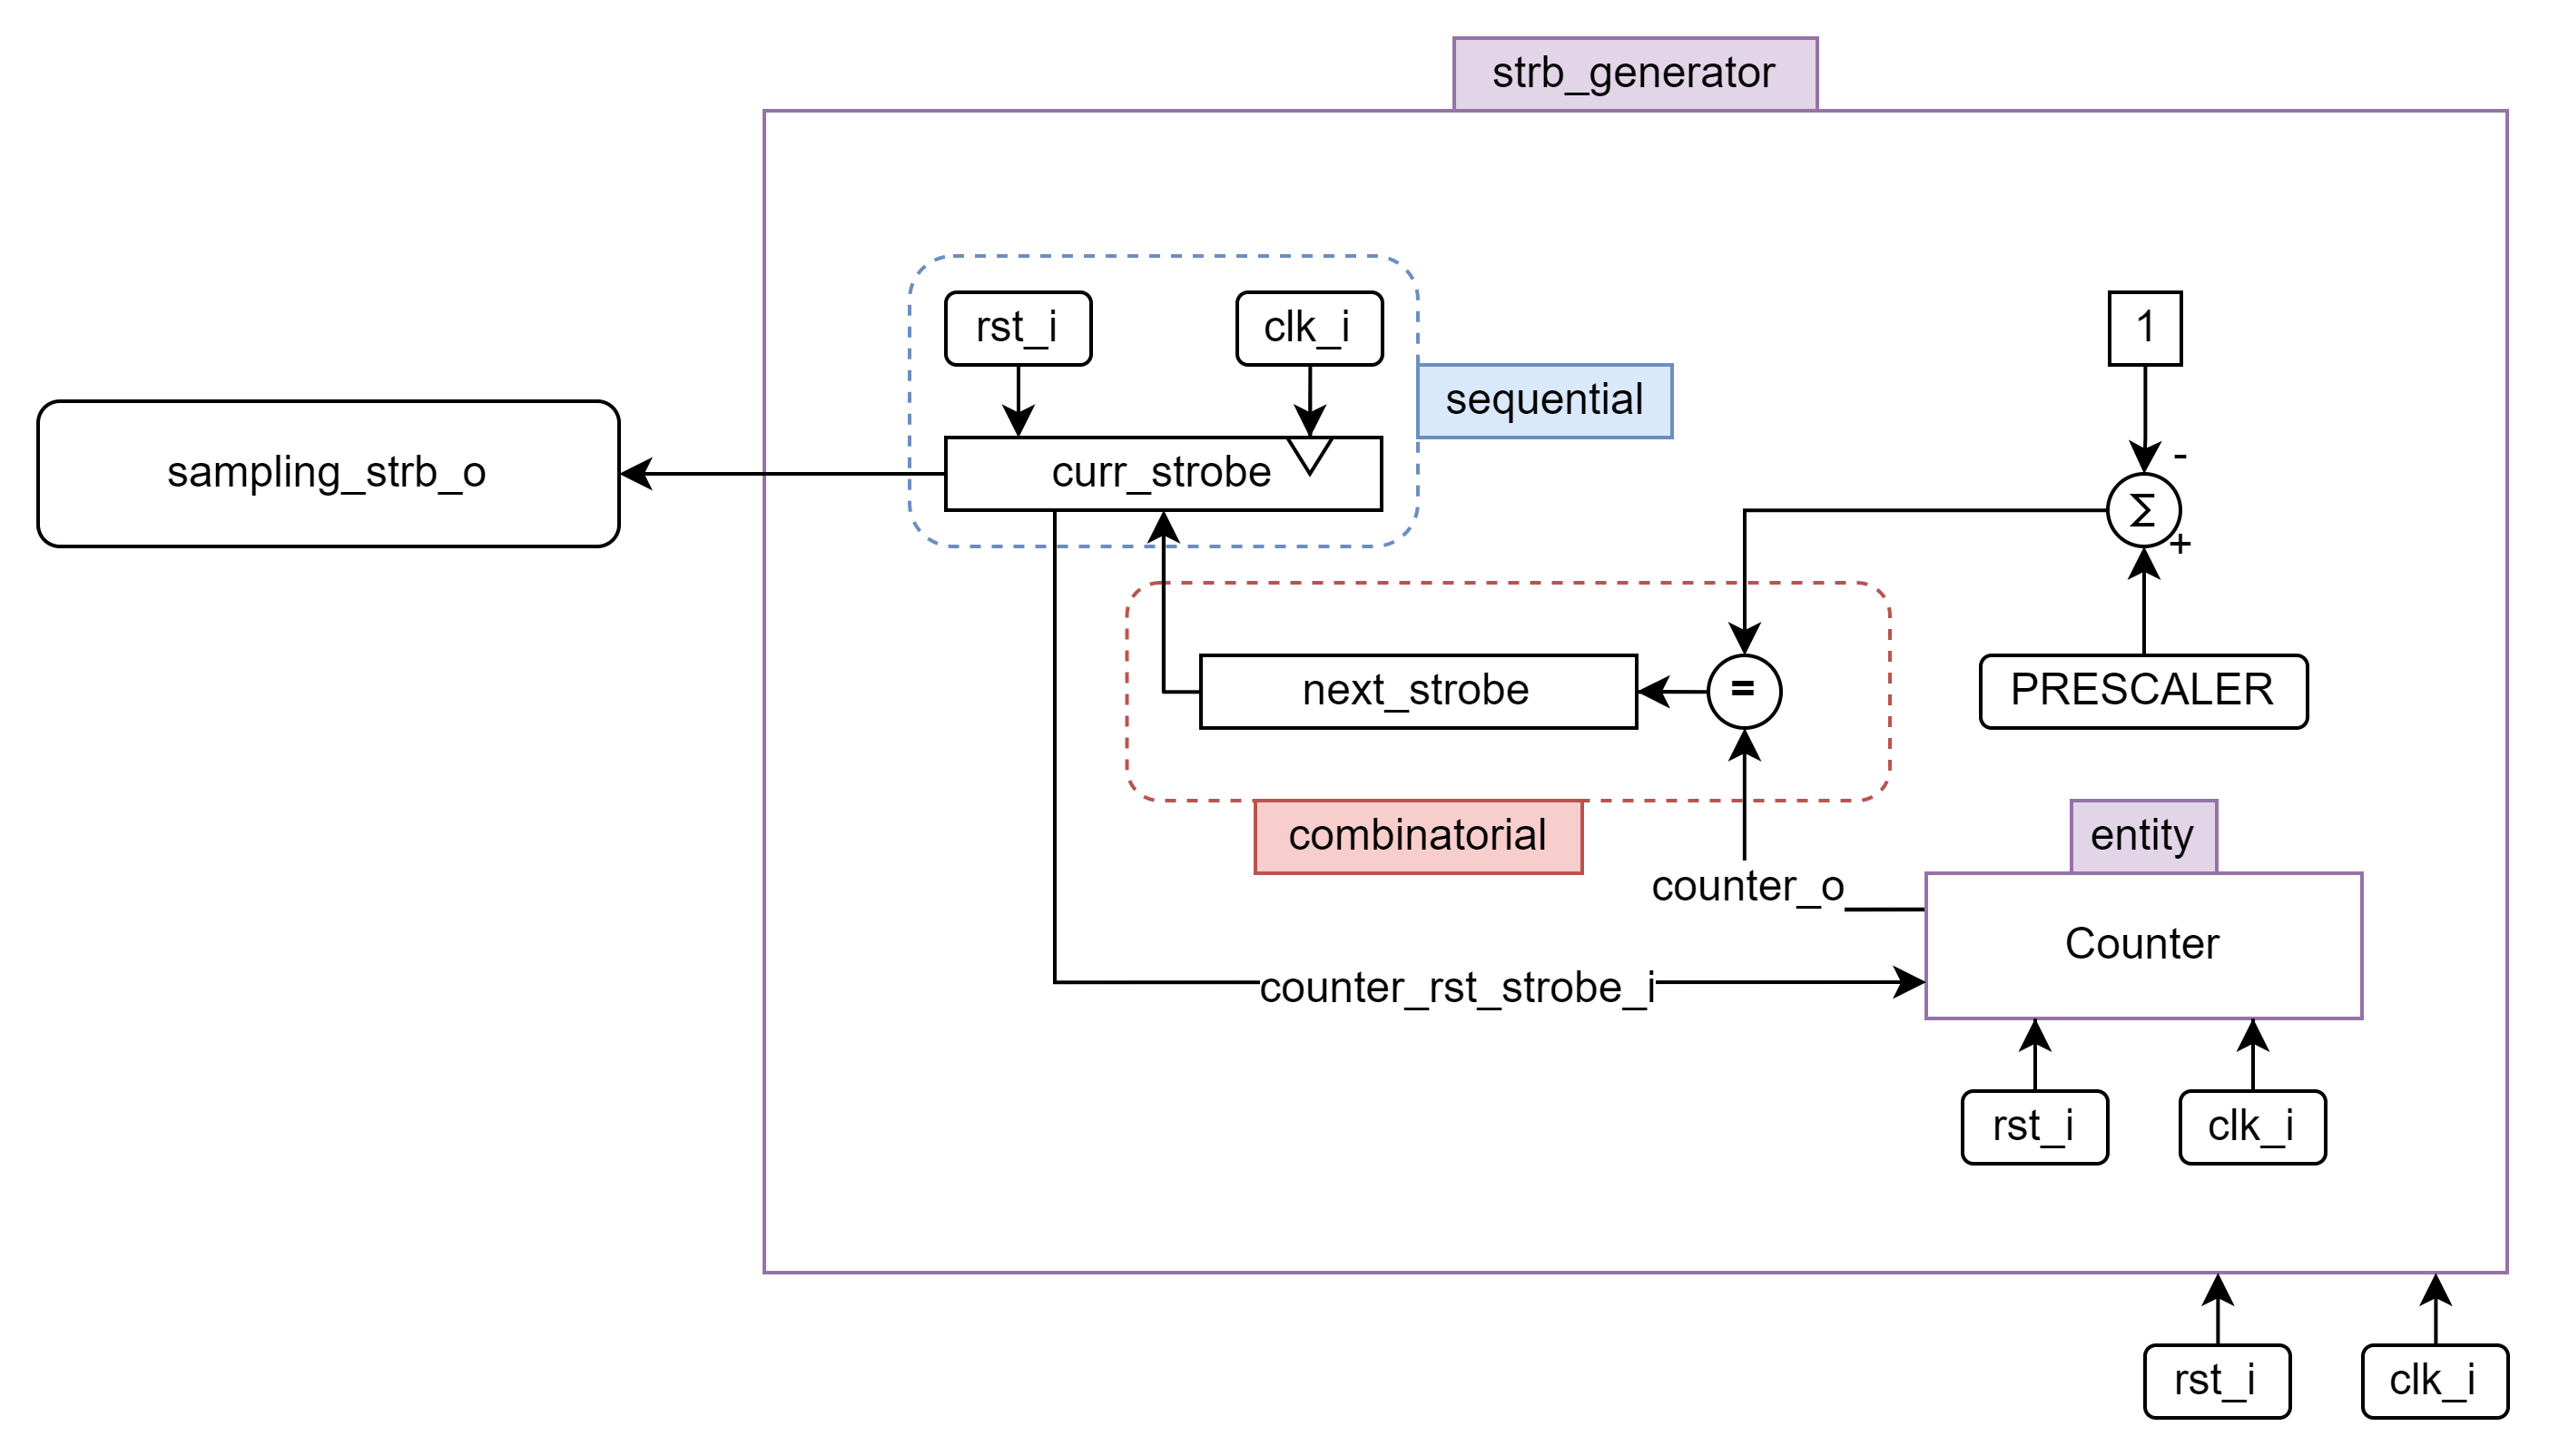
\includegraphics[width=1\linewidth]{images/3_STRB.png}
\end{center}

\textbf{Entity}\hrulefill

%\input{code/strb_e}

\textbf{Architecture}\hrulefill

Bei dieser Realisierung des Strobe-Generators wurde entschieden, dass die
Frequenz, mit der die Strobe Generiert wird keine Zeitdauer, sondern ein Teiler
(Prescaler) der Clock ist. Damit kann der sowieso Notwendige Counter auch für
die Abzählung der Sampling-Periode verwendet werden. 

Signale

\begin{lstlisting}
signal next_strobe : std_ulogic := '0';
signal curr_strobe : std_ulogic := '0';
signal strb_counter : unsigned(PRESCALER-1 downto 0) := (others => '0');
\end{lstlisting} 

\newpage

(1) \lstinline{reg_seq : process (clk_i, rst_i)} 

\begin{quote}
    Der sequenzielle Prozess bestimmt das Clock- und Resetverhalten. Bei der
    steigenden Flanke wird der momentanen Strobe \lstinline{curr_strobe} dem
    nächsten, kombinatorisch ermittelten Strobe-Zustand \lstinline{next_strobe}
    zugewiesen. Beim Reset wird der Strobe-Ausgang auf \lstinline{'0'} gesetzt. 
\end{quote}

(2) \lstinline{strb_comb : process (strb_counter)}

\begin{quote}
    In diesem Prozess wird die Kombinatorik zur Bestimmung des nächsten
    Strobe-Zustands beschrieben. Standardmäßig ist der nächste Strobe Zustand
    \lstinline{'next_strobe'} gleich \lstinline{'0'}. Erreicht der
    Strobe-Counter jedoch seinen maximalen Wert, wird \lstinline{next_strobe '1'}.
    Da die Reset-Strobe des Counters mit \lstinline{curr_strobe}
    verbunden ist, wird \lstinline{next_strobe} zurück auf \lstinline{'0'}
    gesetzt. Damit wird erreicht, dass der Strobe-Ausgang genau für eine
    Periode High ist.
\end{quote}

\subsection*{Simulation}

\textbf{Strobe Test} \hrulefill

Hier ist das Strobe-Signal mit einem Prescaler von 10 zu sehen, wie es nach 10 Taktflanken für eine Periode lang high wird.

\begin{center}
    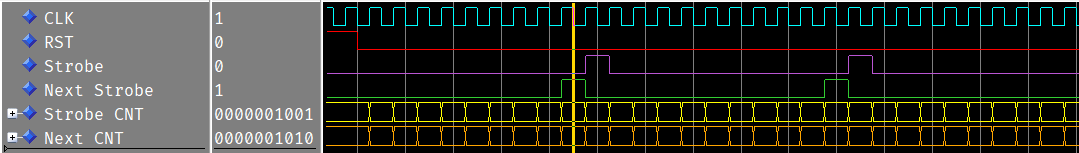
\includegraphics[width=1\linewidth]{images/SIM_STRB1.png}
\end{center}

Hier ist die Ermittlung der Counter Länge nicht optimal, da sie durch
\lstinline{unsigned(PRESCALER-1 downto 0)} bestimmt wird. Die größe des Counter
Wertes ist daher viel zu groß, da nur bis zum Prescaler Wert gezählt wird und
nicht bis $2^{10}$. Man müsste den Prescaler entweder als
\lstinline{std_ulogic_vector} übergeben, oder eine art log2 Funktion
implementieren.

\newpage
